

\section{Best-fit parameters}
After running multiple simulations as discussed in section 4.4, the current set of best parameters for our model are shown in the table below
\begin{table}[!hbt]
	\centering
	\begin{tabular}{|c|c|c|c|c|c|c|c|c|c|c|c|}
		\hline
		$\mathbf{k_b}$&  $\mathbf{k_{ub}}$ &  $\mathbf{c_b}$&  $\mathbf{c_m}$& $\mathbf{c_t}$ & $\mathbf{\ell_s}$ & $\mathbf{\ell_t}$ & $\mathbf{r_t}$ & $\mathbf{r_m}$ &$\mathbf{r_b}$ & $\mathbf{dt}$ & $\mathbf{c}$\\  
		$s^{-1}$ & $s^{-1}$ & $k_bT$ & $k_bT$ & $k_bT$& nm & nm & nm & nm & nm & $s$ &  \\
		\hline \hline
		$9.5e9$ & $1e20$ & $0.08$ & $1.05$ & $0.36$ & $20.75$ & $23.0$ & $6.0$ & $5.5$ & $1.75$ & $1e10$ & $0.35$\\ 
		\hline
	\end{tabular}
\caption[Best parameters]{Current set of best fit parameters}
\label{table:params}
\end{table}

With these parameters, the following analysis was performed for multiple simulations with a variety of different random number seeds. 



\section{Stepping}

Our model is able to achieve directed motion with clear evidence of the desired Brownian jiggling. All simulations show a net displacement in the positive x direction.
\begin{figure}[!hbt]
	\centering
	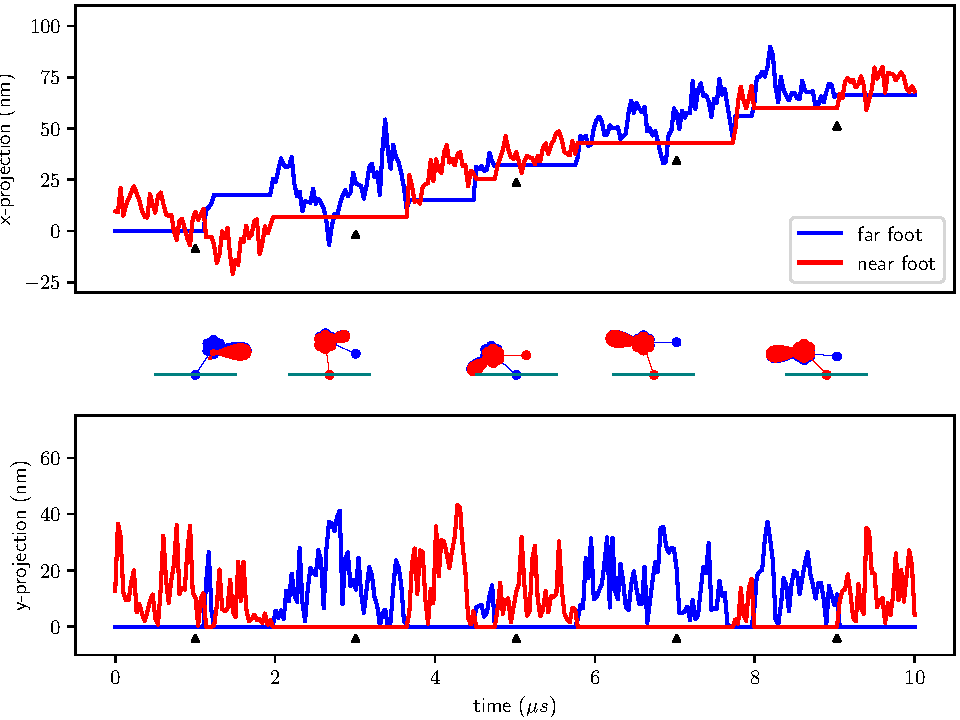
\includegraphics[width=1\columnwidth]{paper_trajectory_plot}
	\caption[Trajectory plot]{\textbf{Trajectory Plot} for a small subset of steps. Vertical and horizontal projections for the trajectory of each binding domain are plotted in red and blue. Directed motion is clearly seen in the positive slope of the x-projection graph. Dynein's conformation is illustrated for a selection of times.}
	\label{fig:trajectory}
\end{figure}

As y-projection plot in figure \ref{fig:trajectory} indicates, the model performs a wide diffusive search for the microtubule, assuming a wide range of configurations along the way. The cartoons corresponding to the black triangles in the x and y projection plots show the motor domains travel around the tail linker during the stepping cycle. This behavior is suggestive of the power-stroke model proposed by \cite{burgess2003dynein} and others. It is also worth noting that the y-projection plot suggests an average binding domain height $>0$. This is contrary to the popular depictions of dynein with the binding domains nearly scrubbing the microtubule until binding.\\

Dynein's stepping velocity can be seen in the positive slope of figure \ref{fig:trajectory}. This velocity is directly related to the stepping rates. To increase the model's velocity, simply increase both the binding and unbinding rates. \\ 

Running a longer simulations at multiple random number seeds allows us to gather more stepping statistics. A sample of these are shown in figure \ref{fig:statistics}. 
	
\begin{figure}
	\centering
	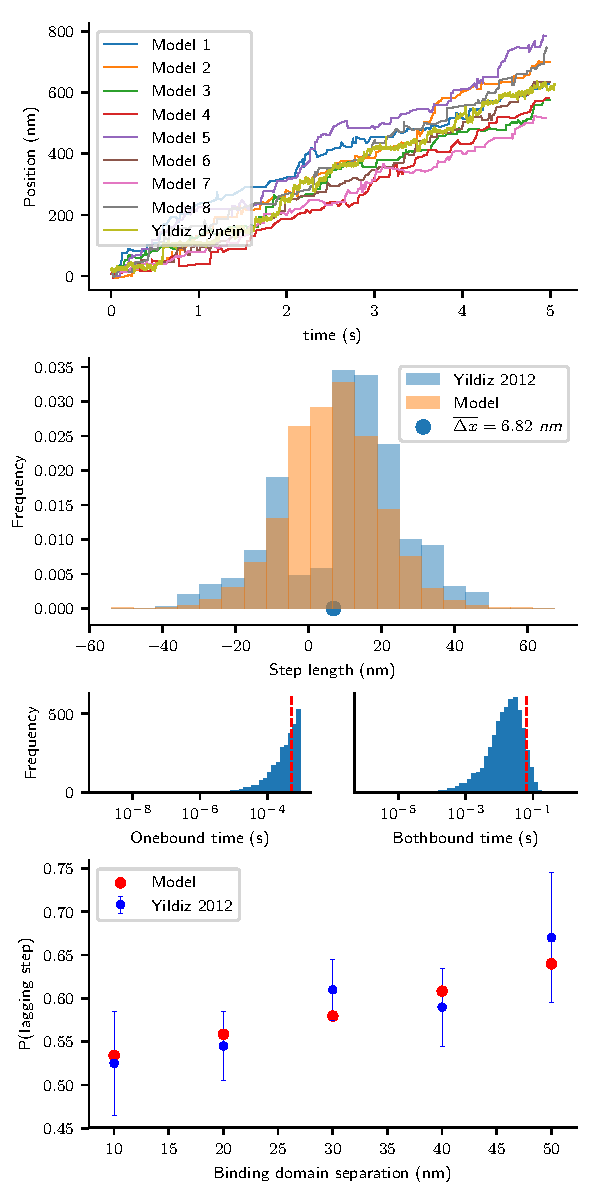
\includegraphics[width=0.85\columnwidth]{paper_model_behavior}
	\caption[Model Stepping Statistics]{\textbf{Stepping statistics} trajectories run with different random number seeds all show forward directed motion. Step lengths have a similar distribution to experiment although steps of zero length are not measured experimentally. }
	\label{fig:statistics}
\end{figure}


The first graph in figure \ref{fig:statistics} shows the x position trajectory plot for the same simulation run with many different random seeds. An experimental trajectory plot is shown in blue with data taken from \cite{dewitt2012cytoplasmic}. This figure illustrates that even for long simulations, the model shows directed motion despite occasionally stepping backwards. Furthermore, we can see that average velocity across each of the model simulations agrees well with the experiment. 

The second graph in figure \ref{fig:statistics} shows a signed step length histogram comparing the model with data from \cite{qiu2012dynein}. Here negative values of step length indicate a backwards step. The shape of the histogram matches well with the experiment despite missing the notable dip at zero step length. This is likely due to the fact that a step of zero length (i.e. a stutter step) can not be distinguished experimentally from the typical Brownian motion. \\ 

Finally, we plot histograms for the time spent in the one bound and both bound states during each simulation. The red line indicates our estimates for these values based off of experimental stepping velocities. It is interesting to note that in both cases, the average time spent in each state is below this estimate. Despite this, we can clearly see that the median one bound time is around $0.0015-0.003$ seconds while the both bound time is between lies somewhere between $0.015-0.03$ seconds-- an order of magnitude higher. This suggests that dynein spends most of its time in the both bound state. 


\section{State correlations}
If the both bound time is significantly higher than the one bound time, perhaps the two states are uncorrelated. In other words, does our model predict that the configuration of dynein before a step is unrelated to the final configuration when it rebinds again? To investigate this possible result, we plot the initial displacement versus the step length for the steps taken during all of the simulations. We consider these quantities as signed distances. For the step length, this indicates whether or not the model steps forwards or backwards. For the initial displacement, the sign indicates which binding domain initiates the step as indicated in the following figure. 
\begin{figure}[!hbt]
	\centering
	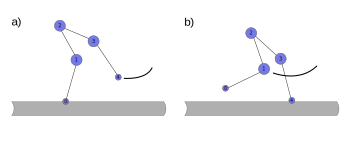
\includegraphics[angle=-90, width=1\columnwidth]{leading_vs_lagging}
	\caption[Leading vs Lagging Steps]{Diagram illustrating a leading foot step (a) and a lagging foot step (b).}
\end{figure}



 
\begin{figure}[!hbt]
	\centering
	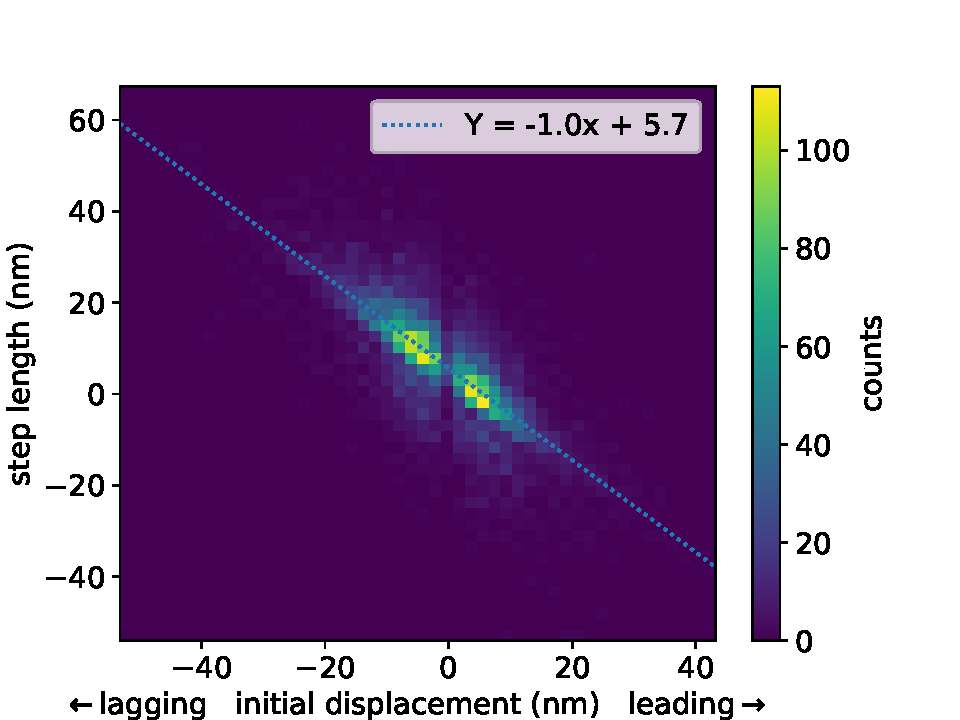
\includegraphics[width=0.75\columnwidth]{paper_displacement_vs_step_length}
	\caption[Initial displacement vs Step Length]{\textbf{Two dimensional histogram} comparing the total signed step length to
			the signed initial displacement between the binding domains. A positive value
			indicates that the front foot made the step (leading). A negative value
			indicates the rear foot (lagging) made the step. Simulations show a strong,
			negative correlation. A similar fit from an experimental paper is plotted for comparison.}
	\label{fig:displacement_vs_step_length}
\end{figure}
	
Figure \ref{fig:displacement_vs_step_length} is a two-dimensional histogram for which step lengths are binned against initial displacements. A linear fit through the data (orange dashed line) indicates that the distribution is shifted vertically. This reflects the model's preference for stepping in the positive direction. Interestingly though, the slope of this fit appears much stepper than the same fit for experimental data from \cite{dewitt2012cytoplasmic}. 

If we define the final step length to be 
\begin{equation}
\text{final displacement} = \text{initial displacement} + \text{step length },
\end{equation}	
then clearly our model indicates that the final displacement is roughly the same regardless of the initial displacement-- a conclusion at odds with the experimental data. This discrepancy may be due to the low number of data points in \cite{dewitt2012cytoplasmic}, but it can not be explained away by the expected lack of zero nm step observations. 


\section{Simulating states separately}
Our simulations appear to predict that the one bound and both bound states are uncorrelated with each other. Therefore, one reasonable conclusion is: Why simulate them together in the first place? \\

We are now developing a simplified simulation code for our model which still performs the full Brownian dynamics for the short lived one bound state but takes advantage of this result by removing the both bound portion of the simulation all together. Instead, we seek to use Monte Carlo methods to generate both bound stepping statistics by determining unbinding based on the distribution of possible both bound configurations for a given initial displacement. \\

\begin{figure}[!hbt]
	\centering
	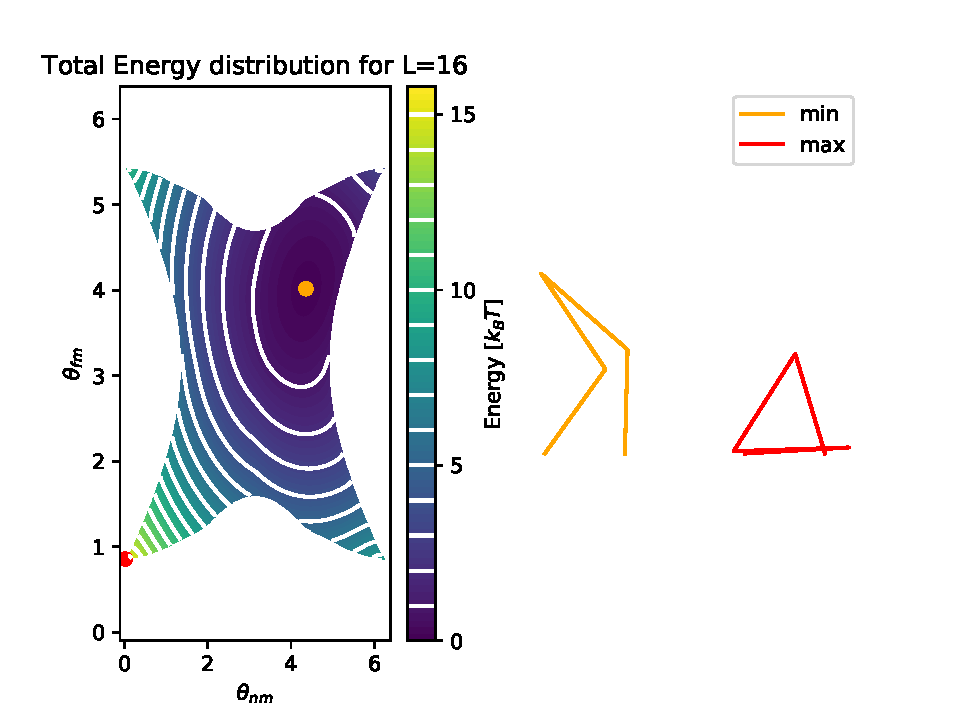
\includegraphics[width=1\columnwidth]{energy_landscape}
	\caption[Energy Landscape]{\textbf{Energy Landscape} graph showing the total energy of the dynein for a given binding domain displacement $L$. The yellow and red dots correspond to the minimum and maximum energy configurations for which a cartoon is shown on the right.}
	\label{fig:energy_landscape}
\end{figure}
In figure \ref{fig:energy_landscape} we can see a contour plot of the energy associated with dynein in the both bound state for all possible allowed combinations of near motor and far motor angles given an interhead separation of $16$ nm. Indicated on the graph are the minimum and maximum energy configurations (orange and red respectfully). The total energy appears to increase monotonically outwards from the minimum suggesting that the orange configuration shown to the right of the figure is a reasonable representative for the typical both bound state with this interhead separation. 

We anticipate that a simulation distinguishing between the two states will significantly improve the computation time and enable us to fit simulation parameters more tactfully. 
			

\vspace{10em}
